%%%%%%%%%%%%%%%%%%%%%%%%%%%%%%%%%%%%%%%%%%%%%%%%%%%%%%%%%%%%%%%%%%%%%%%%%%%%%%%%
%2345678901234567890123456789012345678901234567890123456789012345678901234567890
%        1         2         3         4         5         6         7         8

\documentclass[letterpaper, 10 pt, conference]{ieeeconf}  % Comment this line out if you need a4paper

%\documentclass[a4paper, 10pt, conference]{ieeeconf}      % Use this line for a4 paper

\IEEEoverridecommandlockouts                              % This command is only needed if 
                                                          % you want to use the \thanks command

\overrideIEEEmargins                                      % Needed to meet printer requirements.

%In case you encounter the following error:
%Error 1010 The PDF file may be corrupt (unable to open PDF file) OR
%Error 1000 An error occurred while parsing a contents stream. Unable to analyze the PDF file.
%This is a known problem with pdfLaTeX conversion filter. The file cannot be opened with acrobat reader
%Please use one of the alternatives below to circumvent this error by uncommenting one or the other
%\pdfobjcompresslevel=0
%\pdfminorversion=4

% See the \addtolength command later in the file to balance the column lengths
% on the last page of the document

% The following packages can be found on http:\\www.ctan.org
\usepackage{graphics} % for pdf, bitmapped graphics files
\usepackage{epsfig} % for postscript graphics files
\usepackage{mathptmx} % assumes new font selection scheme installed
\usepackage{times} % assumes new font selection scheme installed
\usepackage{amsmath} % assumes amsmath package installed
\usepackage{amssymb}  % assumes amsmath package installed
\usepackage[latin1]{inputenc}

% Bildumgebungen
\usepackage{graphicx}
\graphicspath{{picture/}}
\usepackage{import}
\usepackage{xcolor}

\usepackage{blindtext}
\usepackage{url}




\title{\LARGE \bf
Developement of an autonomous driving environment model visualization based on object list level
}


\author{Tobias Wagner  Christoph Zach Max Haindl Philipp Korn Stehpan ...? Dennis Roessler Max Pfaller Domi ...? % <-this % stops a space
\thanks{*This work was not supported by any organization}% <-this % stops a space

}


\begin{document}



\maketitle
\thispagestyle{empty}
\pagestyle{empty}


%%%%%%%%%%%%%%%%%%%%%%%%%%%%%%%%%%%%%%%%%%%%%%%%%%%%%%%%%%%%%%%%%%%%%%%%%%%%%%%%
\begin{abstract}

This electronic document is a live template. The various components of your paper [title, text, heads, etc.] are already defined on the style sheet, as illustrated by the portions given in this document.

\end{abstract}


%%%%%%%%%%%%%%%%%%%%%%%%%%%%%%%%%%%%%%%%%%%%%%%%%%%%%%%%%%%%%%%%%%%%%%%%%%%%%%%%
\section{INTRODUCTION}


\section{RELATED WORKS}

IEEE Fabio Reway Test Method for Measuring the Simulation-to-Reality Gap of Camera-based Object Detection Algorithms for Autonomous Driving


\section{MATERIALS AND METHODS}

Kleines Intro was jetzt kommt


\begin{figure}[thpb]
      \centering
       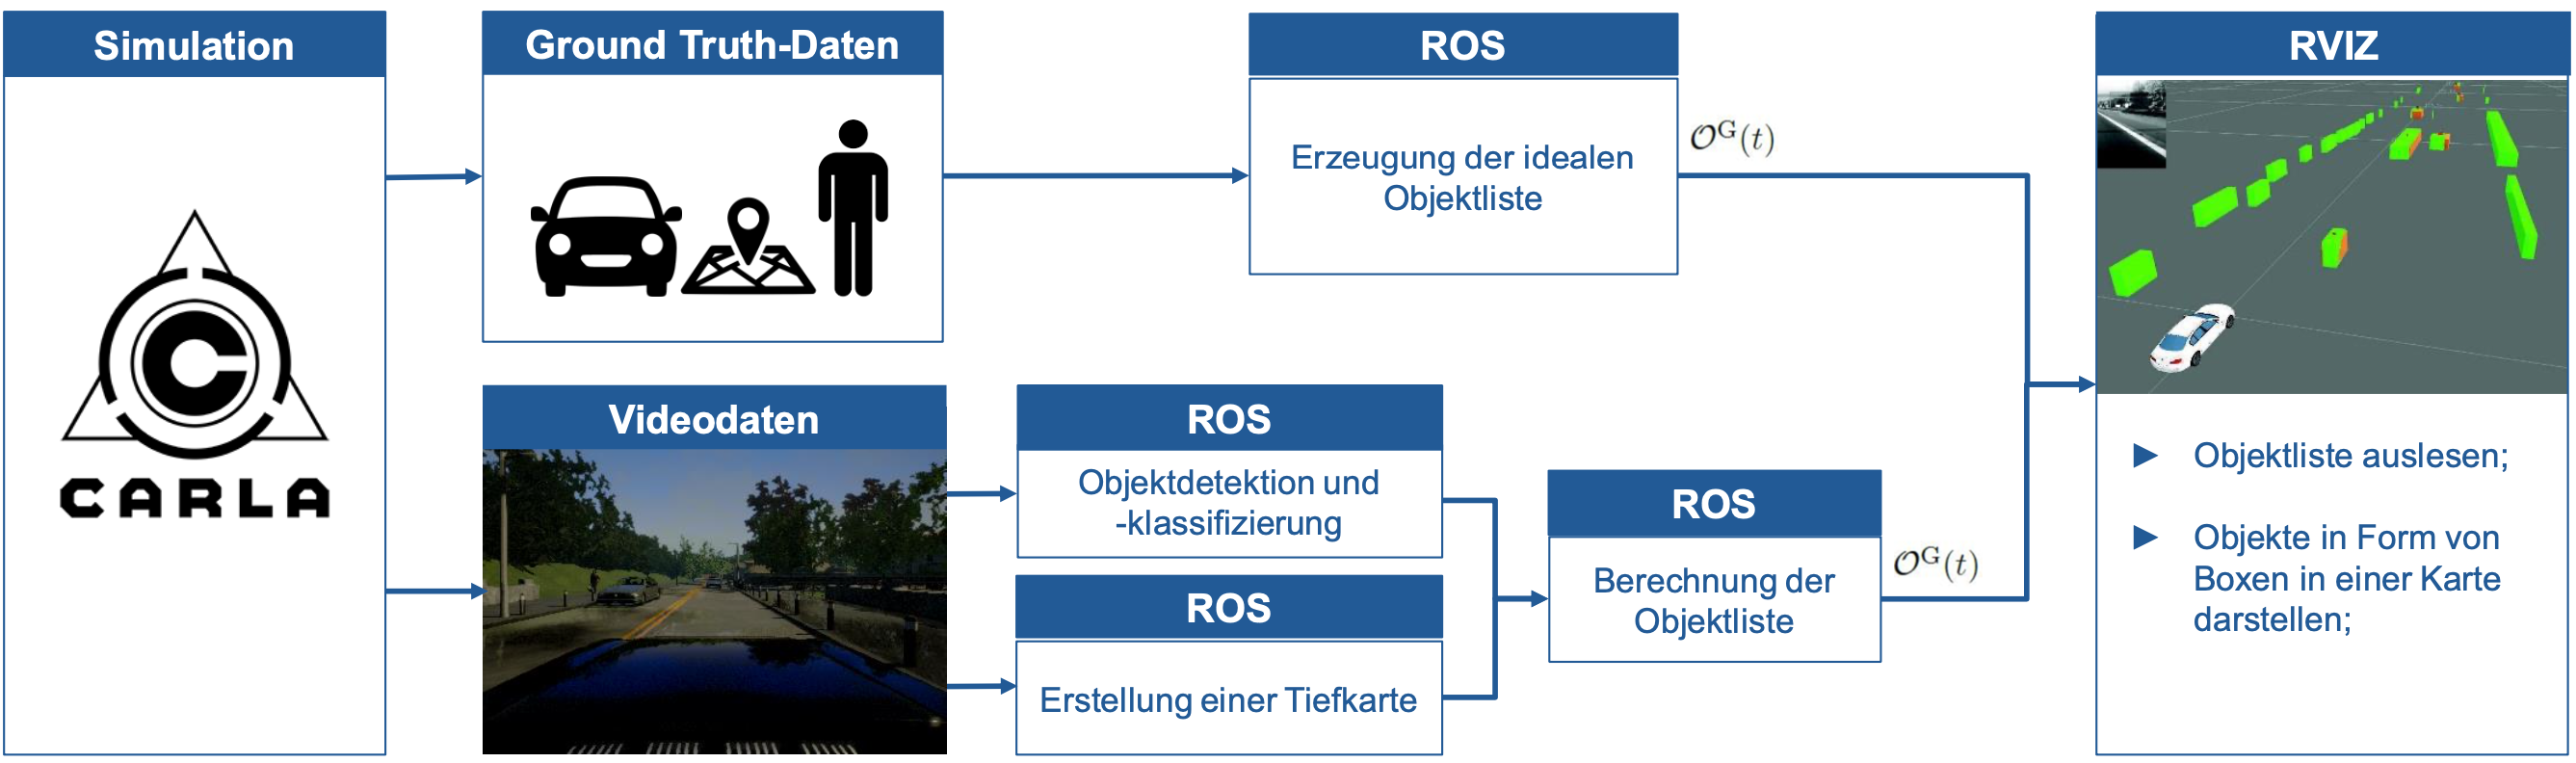
\includegraphics[scale=0.17]{Ueberblick}
      \caption{Ueberblick }
      \label{figurelabel}
   \end{figure}
\subsection{Creating simulation scenario}

\begin{itemize}
\item Welcher Simulator wurde verwendet
\item Welches Szenario (NCAP)
\item Szenario beschreiben
\end{itemize}


   
\subsection{Creating objects list of ground-truth data (TP1}

\begin{itemize}
\item Erstellung Objektliste
\item Objektliste anhand Attribut-Vektor beschreiben
\item Ros-System beschreiben
\item Feature Vektor Ermittlung
\end{itemize}

   \begin{figure}[thpb]
      \centering
       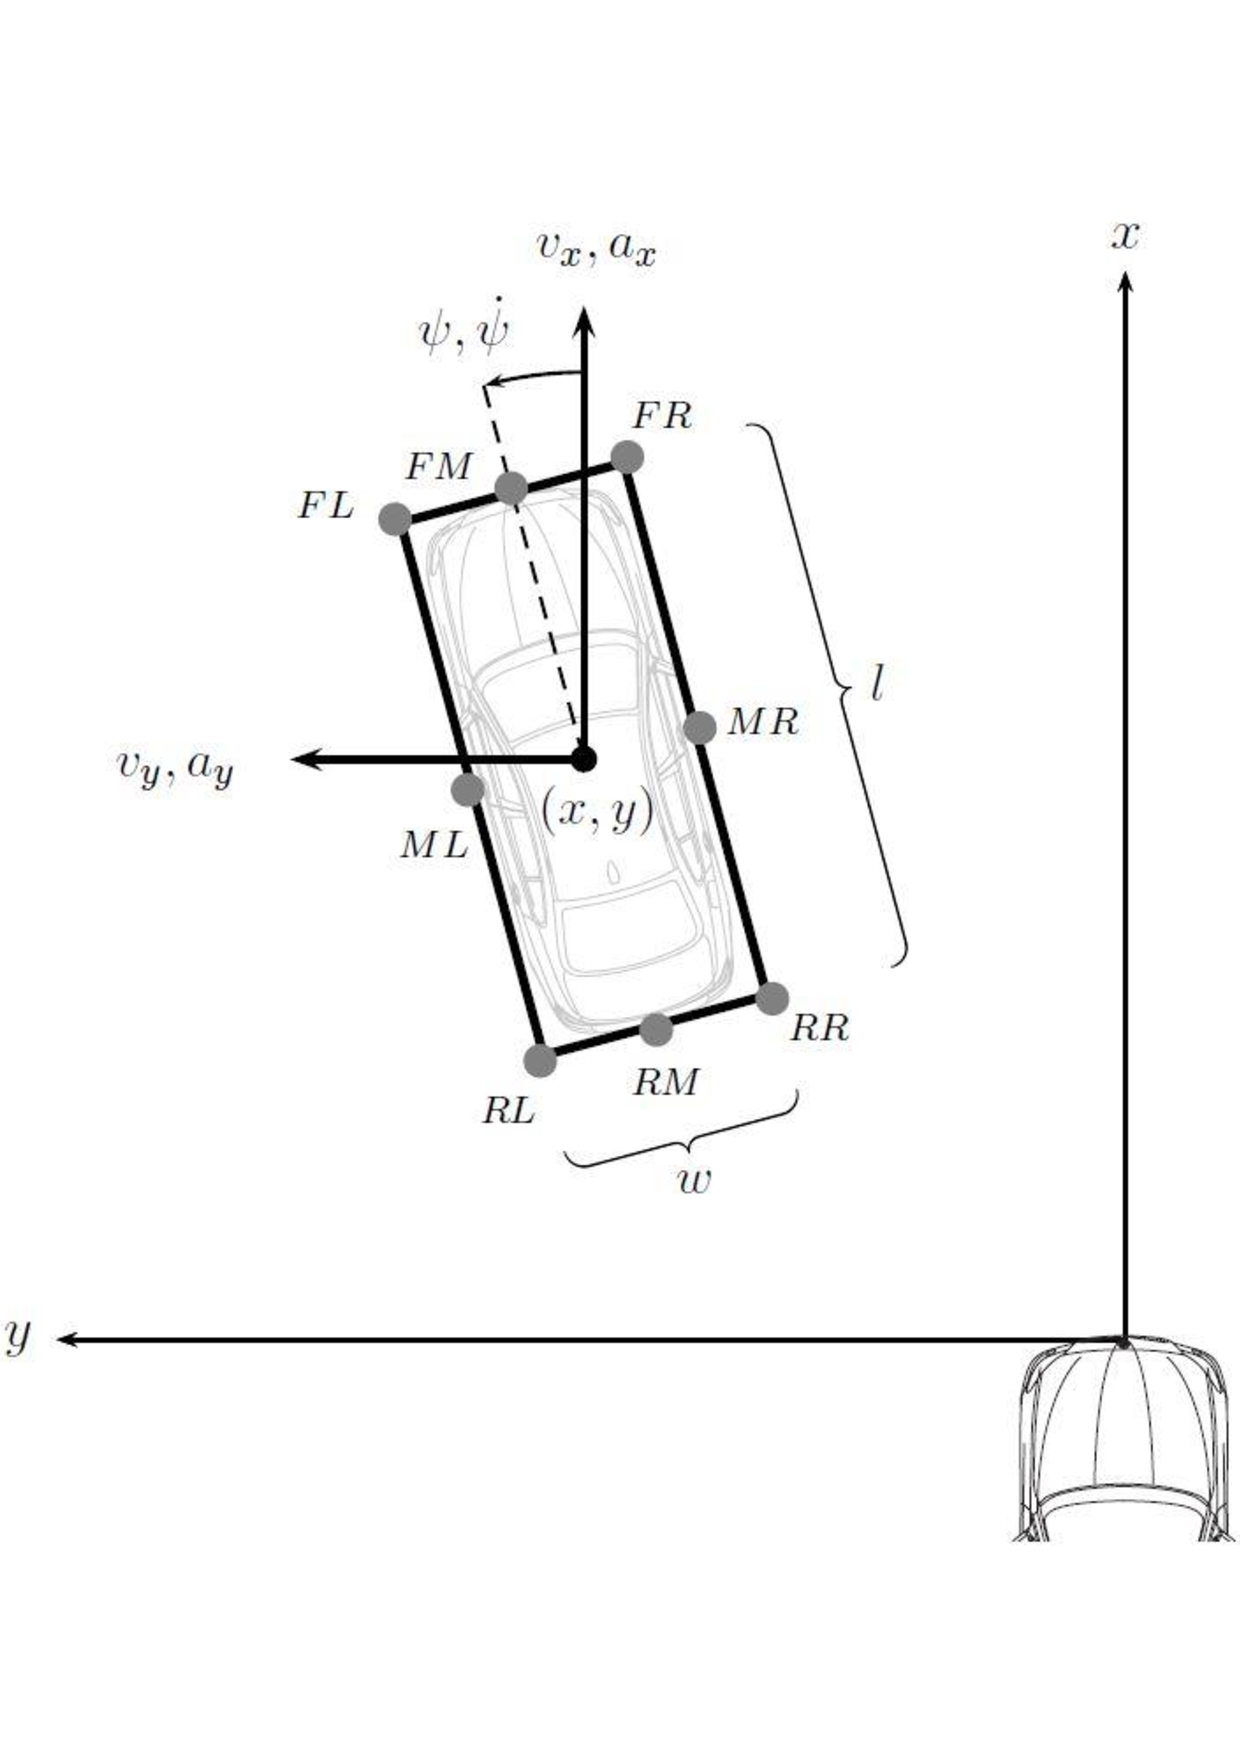
\includegraphics[scale=0.3]{KoordinatenSystem}
      \caption{Fahrzeugkoordinatensystem}
      \label{figurelabel}
   \end{figure}
\subsection{Evaluation of video data (TP2)}

\begin{itemize}
\item Detektion Objekte (Yolo)
\item Tracking Objekte (Tracker)
\item Gleichung zur Berechnung von zB Geschwindigkeit, Beschleunigung
\item Ermittlung Classification / prop mov / prop exis

\end{itemize}

\subsection{Visualization of object lists(TP3)}
%Die erzeugten Objektlisten aus den groundtruth Daten bzw. Videodaten werden über ROS veröffentlicht. 

\begin{itemize}
\item subscription der Objektlisten
\item Auswertung der Objektlisten,Marker Array, Tf Transform, 



\end{itemize}

\subsection{Evaluation of object lists(TP3)}

\begin{itemize}
\item Objektlisten in BagFiles aufnehmen
\item Geo und Time mapping
\item Berechnung von iOu etc. verweis auf Veröffentlichung von Fabio




\end{itemize}

\section{RESULTS}

Ergebnisse des Projekts:
 
 \begin{itemize}
\item Funktioniert die Auswertung
\item Wie gut sind die Kamerawerte im Vergleich zu Groundtruth Werte
\item sind die Werte represenativ
\end{itemize}













   
\section{CONCLUSIONS}



\addtolength{\textheight}{-12cm}   % This command serves to balance the column lengths
                                  % on the last page of the document manually. It shortens
                                  % the textheight of the last page by a suitable amount.
                                  % This command does not take effect until the next page
                                  % so it should come on the page before the last. Make
                                  % sure that you do not shorten the textheight too much.


\section*{APPENDIX}



\section*{ACKNOWLEDGMENT}



\bibliographystyle{IEEEtran}{
\bibliography{ref/ref_list.bib}}


\end{document}
